%=================================================================
\section{Introduction}\label{sec-intro}


%Test citation~\cite{BL12J01}. 
%\begin{JournalOnly}
%and~\citep{BJL11J01} or~\citet{BJL11J01}.
%\end{JournalOnly}

%This is for~\cref{tbl:overall-experiments}, 
%\todo[fancyline]{Testing.}
%and this is for~\cref{sec-conclusions}.
%\todo[noline]{A note with no line back to the text.}%
%\gangli{This is comment from Gang.}
%\qwu{Response from QW}

%Number:
%\num{123}.
%\numlist{10;30;50;70},
%\numrange{10}{30},
%\SIlist{10;30;45}{\metre},
%and
%\SI{10}{\percent}

%\missingfigure[figcolor=white]{Testing figcolor}
\subsection{Problem Statement}
\

You are given 5 years of store-item sales data, and asked to predict 3 months of sales 
for 50 different items at 10 different stores.
\subsection{Data List}
\

The data contains date of the item sold at a store ,And the name of the store,And the name of the item,
and the sales of every store on a particular day.
\begin{description}
  \item [date] - Date of the sale data. There are no holiday effects or store closures.
  \item [store] - Store ID.
  \item [item] - Item ID.
  \item [sales] - Number of items sold at a particular store on a particular date.
\end{description}

\subsection{Problem Analysis}
\

This is a question that asks us to predict sales for three months
 based on sales that have been available for three years. And We can
 analyze that this is a regression problem.

\section{Exploratory Data Analysis} \label{sec-data_exploration}

\subsection{Data Information}
\

From the table 1, we can clearly understand the situation of the 
data set. And we can see the sales volume and sales time of each 
product in each store during the term of 2013-1-1 to 2017-12-31.

\begin{table}[htbp]  \centering
	\caption{Data Information}
	\label{tbl:data information}
	\begin{tabular}{ccccccc}
		\hline
		% after \\: \hline or \cline{col1-col2} \cline{col3-col4} ...
		& date & store & item & sales\\
		\hline
		0 & 2013-01-01 & 1 & 1 & 13 \\
	  1 & 2013-01-02 & 1 & 1 & 11 \\
		2 & 2013-01-03 & 1 & 1 & 14 \\
		3 & 2013-01-04 & 1 & 1 & 13 \\
	  4 & 2013-01-05 & 1 & 1 & 10 \\
		\hline 
		%\bottomrule
	\end{tabular}
\end{table}

\subsection{Data Visualization}
\

By using the matplotlib to plot the photoes which describe the
sale pattern. For example, The distribution of sales volume ,total 
sales of the stores, total sales of the items, store’s performance 
over the time, all items’ performance over the time ect.

From the figures 1 we can know that 2nd store is the topper and
7th store is the least revenue generating one; From figure 2 we can
know that more and more sales volume is belong to [0,50]; From figure 
3 we can know that 2nd store is the topper of the all stores; From
figure 4 we can know the total sales of all items; From figure 5 we 
can know every stores sales changing overtime; From figure 6 we can
know every item sales changing overtime; From figure 7 and 8 we can 
know individual pattern of item’s sale and store’s sale.

\begin{figure}[htbp]
	\centering
	
	%\graphicspath{{figures/}{mine/}}
	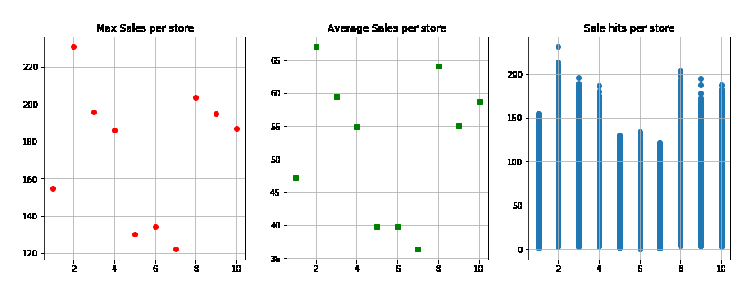
\includegraphics[scale=0.8]{logos/0003.eps}
	\caption{Displaying the sale pattern}\label{fig:001.eps}
\end{figure}

\begin{figure}[htbp]
	\centering
	
	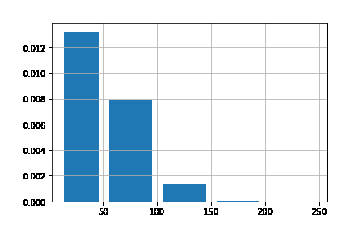
\includegraphics[scale=0.8]{logos/0004.eps}
	\caption{ sales volume’s distribution}\label{fig:002.eps}
\end{figure}

\begin{figure}[htbp]
	\centering
	
	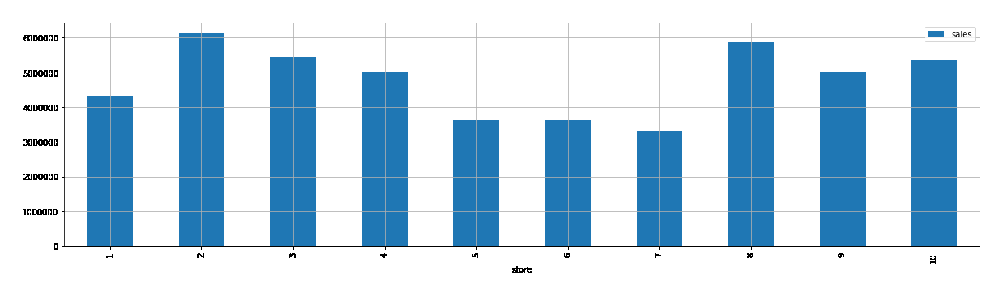
\includegraphics[scale=0.6]{logos/0005.eps}
	\caption{ The total sales of all stores}\label{fig:003.eps}
\end{figure}

\begin{figure}[htbp]
	\centering
	
	\includegraphics[scale=0.3]{logos/0006.eps}
	\caption{ The total sales of all items}\label{fig:004.eps}
\end{figure}

\begin{figure}[htbp]
	\centering
	
	\includegraphics[scale=0.3]{logos/0007.eps}
	\caption{  The performance of all stores}\label{fig:005.eps}
\end{figure}

\begin{figure}[htbp]
	\centering
	
	\includegraphics[scale=0.3]{logos/0008.eps}
	\caption{ The performance of all stores items}\label{fig:006.eps}
\end{figure}

\begin{figure}[htbp]
	\centering
	
  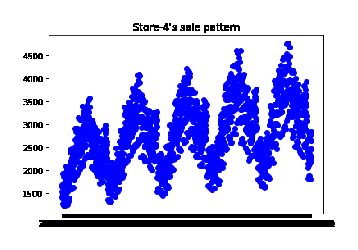
\includegraphics[scale=0.7]{logos/0009.eps}
  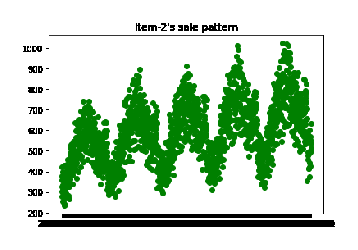
\includegraphics[scale=0.7]{logos/0010.eps}
	\caption{  The performance of the individual store and item}\label{fig:007.eps}
\end{figure}

\subsection{Data Preparation}
\ 

Through the data visualization before, we can intuitively 
recognize the changes in sales. However, to forecast sales for the 
next three months, we need to extract some new features. From the
previous figure we can see that the sales are related to the 
characteristics of the year, month, season, etc., so we can add some 
new features.

The new features that are specifically added are as follows:
\ 
\begin{description}
  \item [dayofweek] -  Indicates that this day is the day of the week. Monday is \hspace*{1.8cm} indicated by 0, Tuesday is indicated by 1, and so on.
                       Sunday \hspace*{1.8cm} is indicated by 6.
  \item [is\_weekend] - Determine if this day is a weekend. The weekend is indicated \hspace*{1.85cm} by 1 and the working day is represented by 0.
  \item [day] - Judging this day is the first few days of this month.
  \item [year] - Judging year.
  \item [dayofyear] - Judging that day is the first few days of the year.
  \item [weekofyear] - Judging that the day is the first few weeks of the year.
  \item [sales\_mean\_lag\_90] - Calculate 90 days from the day before, and then start \hspace*{3.1cm} from this day, the average of the first 
  seven days.
  \item [sales\_std\_lag\_90] - Calculate 90 days from the day, and then start from this \hspace*{2.7cm} day, the standard deviation of the 
  first seven days.
\end{description}

\section{Methods}

There are many machine learning methods for solving regression problems. This moment I will chose the lightGBM model.

\subsection{Trainning model}
\ 

The lightGBM is light Gradient Boosting Machine which is a gradient boosting framework that uses tree based learning algorithms. 
\ 

It is designed to be distributed and efficient with the following advantages:
\ 

\begin{description}
  \item  Faster training speed and higher efficiency.
  \item  Lower memory usage.
  \item  Better accuracy.
  \item  Support of parallel and GPU learning.
  \item  Capable of handling large-scale data
\end{description}
\ 

Select all the features except for the target variable. And Train LightGBM model.
\subsection{ Evaluate model}
\

Verify the training results using the smape model. Smape is Symmetric Mean Absolute Percentage Error.
\ 
\[SMAPE=\frac{100\%}{n}\sum_{t=1}^n\frac{|F_t-A_t|}{(|A_t|+|F_t|)/2} \]
%\begin{ConferenceOnly}
%We have \SI{10}{\hertz},
%\si{\kilogram\metre\per\second},
%the range: \SIrange{10}{100}{\hertz}.
%$\nicefrac[]{1}{2}$.

%\missingfigure{Make a sketch of the structure of a trebuchet.}

%\end{ConferenceOnly}


%For~\cref{eq:test},
%as shown below:

%\begin{equation}\label{eq:test}
%a = b \times \sqrt{ab}
%\end{equation}

%\blindmathpaper

\section{Experiment and Analysis}

First i divide training data and test data by using sklearn, and 
then i do a model training. The next step is model prediction, and 
then i do a model evaluation by using SMAPE. Third, re-train the 
model and the Feature importances will be get. Last ,I will make test predations

\begin{figure}[htbp]
	\centering
	
  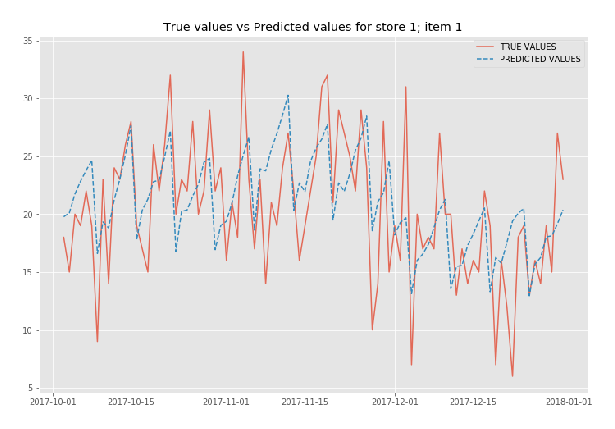
\includegraphics[scale=0.5]{logos/012.eps}
	\caption{  The value vs predict}\label{fig:008.eps}
\end{figure}

\begin{figure}[htbp]
	\centering
	
  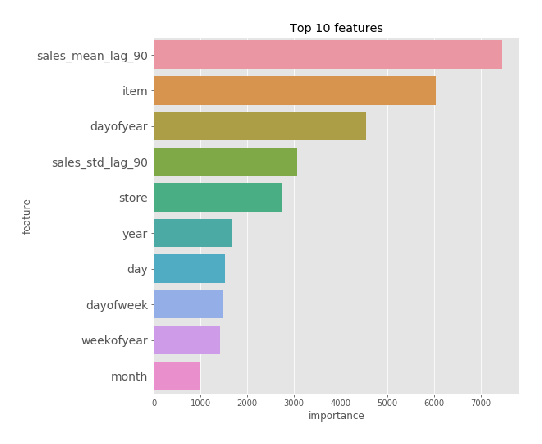
\includegraphics[scale=0.7]{logos/013.eps}
	\caption{Top 10 importabce features }\label{fig:009.eps}
\end{figure}

\begin{figure}[htbp]
	\centering
	
  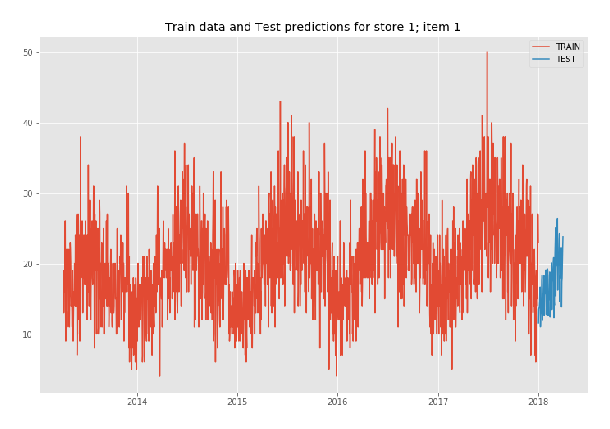
\includegraphics[scale=0.7]{logos/014.eps}
	\caption{ The test prediction }\label{fig:010.eps}
\end{figure}
\ 

ggtgtyfytfyt

Figure 9 is the first prediction based on the model. Figure 10 
shows ten features with high feature importance. Figure 11 is a new
prediction based on the model to get the results needed for this problem.

\section{Conclusion}
\begin{itemize}
	\item[Data Analysis] Using visual methods to find connections and features within the dataset.
	\item[Feature Engineering] Find and extract important features. 
	\item[Modeling] Choose the suitable model parameters.
	\item[Prospcting] I woule like to select multiple models for comparison later.
\end{itemize}
%\section{Preliminaries} \label{sec-preliminaries}

%\blindtext

%\gliMarker  %TODO: GLi Here


%\section{Method} \label{sec-method}

%\blindtext
%\blindlist{itemize}[3]
%\blinditemize
%\blindenumerate

%\blindmathtrue
%\blindmathfalse
%\blinddescription

%\qwuMarker %TODO: QWu Here

%\section{Experiment and Analysis} \label{sec-experiment}


%\begin{table}  \centering
  %\caption{Precision Comparison on Event Detection Methods}
  %\label{tbl:overall-experiments}
  %\begin{tabular}{cccc}
%\toprule
    % after \\: \hline or \cline{col1-col2} \cline{col3-col4} ...
    %& OR Event Detection & AC Event Detection & TC Event Detection \\
%\midrule
    %precision & 0.83 & 0.69 & 0.46 \\
    %recall & 0.68 & 0.48 & 0.36 \\
    %F-score & 0.747 & 0.57 & 0.4 \\
%\bottomrule
%\end{tabular}
%\end{table}


%\section{Conclusions} \label{sec-conclusions}

%\blindtext

%\section*{Acknowledgment}

%\lipsum[1]


%The authors would like to thank \ldots

